\documentclass{beamer}
\usepackage[T2A]{fontenc}
\usepackage[utf8]{inputenc}
\usepackage[english]{babel}
\usepackage{amssymb,amsfonts,amsmath,mathtext}
\usepackage{cite,enumerate,float,indentfirst}
\usepackage[dvips]{graphicx}
\usepackage[linesnumbered,ruled,vlined]{algorithm2e} % NEW

\setbeamertemplate{footline}[page number]

\title[\insertframenumber/\inserttotalframenumber]
{\textbf{Similarity Measures  for \\ Semantic Relation Extraction}}

\author[Alexander Panchenko]
{\textbf{Alexander Panchenko} \\ Université catholique de Louvain (CENTAL) \& \\ Bauman Moscow State Technical University   \\ { \url{alexander.panchenko@uclouvain.be}  }}


\AtBeginSubsection[]
{
  \begin{frame}<beamer>
    \frametitle{Plan}
    \tableofcontents[currentsection,currentsubsection]
  \end{frame}
}

\mode<presentation>
{
%\usetheme{Warsaw}
\usetheme{Singapore}
\usecolortheme{orchid}%whale
\useoutertheme{smoothbars}
%\usefonttheme{serif}
}

\setbeamertemplate{navigation symbols}{%
}

\begin{document}

\begin{frame}
  \titlepage
\end{frame}

\begin{frame}
  \setcounter{tocdepth}{1}
  \frametitle{Plan}
  \tableofcontents
  \setcounter{tocdepth}{2}
	
\end{frame}

\section{Introduction}
\subsection{}

%%%%%%%%%%%%%%%%%%%%%%%%%%%%%%%%%%%%%%%%%%%%%%%%%

\begin{frame}
\frametitle{Goals of the Talk}


\begin{itemize}
  \item Recieve suggestions on how to improve the ML aspects of the work:
  \begin{itemize}
    \item feature selection;
    \item similarity measure learning techniques.
    %\item prior research $[1, 2, 3, 4, 5]$.
   
  \end{itemize}
  \item Interest you in a possible colloborations on:
  \begin{itemize}
    \item application of feature selection to NLP;
    \item semantic similarity measure learning.
  \end{itemize}
\end{itemize}

\end{frame}

%\begin{frame}
%\frametitle{Mainstream NLP methodology:}

%\textbf{Goal:} Build application X.

%\textbf{Solution:}

%\begin{enumerate}
%  \item Collect some training data. 
%  \item \alert{Manually} design features relevant to an application.
%  \item Choose a statistical model and train it on the training data.
%  \item If performance is not enougth: modify 1 or/and 2 or/and 3. 
       
%\end{enumerate}

%\textbf{Practical observations:}
%\begin{itemize}
% \item The biggest improvements are achieved from 2.
% \item Ubiquity of high-dimensional feature spaces in NLP:
% \begin{itemize}
% \item bag of words;
% \item bag of syntactic dependencies;
% \item mix of heterogenous features, \ldots
% \end{itemize} 
% \item Yet most researchers do not consider feature selection. 
%\end{itemize}

%\end{frame}

\begin{frame}



\frametitle{The Problem}

\begin{itemize}
  \item A \textbf{semantic similarity measure}: $s_{ij} = sim(c_i, c_j) \rightarrow [0,1]$
  \begin{itemize}
    \item $c_i, c_j$ -- terms
    %\item 
    $$
  s_{ij} = \left\{ 
   \begin{array}{l l}
     high & \quad \text{if } \langle c_i, c_j \rangle \text{ is a pair of synonyms, hyponyms, etc.} \\
    0 & \quad \text{otherwise}\\
   \end{array} \right.
 $$
    \end{itemize}
  \item Many dissimilar pairs, few similar pairs: $sim(c_i,c_j) \sim exp(\lambda)$
   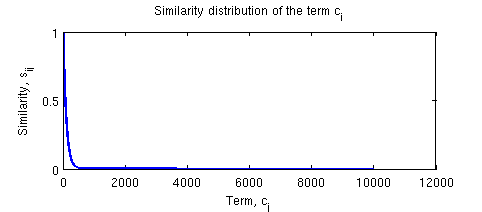
\includegraphics[width=0.6\textwidth]{figures/simdist}
   
     \item Nonnegativity: $s_{ij} \geq 0$;
     \item Reflexivity: $s_{ij} = 1 \Leftrightarrow c_i = c_j$;
     \item Symmetry: $s_{ij} = s_{ji}$;
     \item Triangle inequality: $s_{ij} \leq s_{ik} + s_{kj}$  
   \end{itemize}   
\end{frame}
   
\begin{frame}
\frametitle{Motivation}

\item \textbf{Semantic similarity measures} are useful for NLP/IR:
\begin{itemize}
  \item WSD (Patwardhan et al., 2003)
  \item Query Expansion (Hsu et al., 2006)
  \item QA (Sun et al., 2005)	
  \item Text Categorization (Tikk et al, 2003)
  \item Text Similarity (Šaric et al., 2012)
\end{itemize}

\end{frame}



\begin{frame}
\frametitle{State of the Art}

\begin{itemize}
  \item \textbf{WordNet-based measures}

  \begin{itemize}
  	\item WuPalmer (1994), LeacockChodorow (1998), Resnik (1995)
  	\item rely on manually crafted resources
  	\item highest precision, limited coverage   
  \end{itemize}
  
  \item \textbf{Dictionary-based measures}
	\begin{itemize}
	  \item ExtendedLesk (Banerjee and Pedersen, 2003), GlossVectors (Patward
han and Pedersen, 2006) and WiktionaryOverlap (Zesch et al., 2008)
	\item rely on manually crafted resources
	 \item high precision, limited coverage
	\end{itemize}

\item  \textbf{Corpus-based measures}
\begin{itemize}
  \item ContextWindow (Van de Cruys, 2010), SyntacticContext (Lin, 1998),  LSA (Landauer et al., 1998)
  
 \item no semantic resources are needed
 \item low precision, high recall 
\end{itemize}

\item \textbf{Combined} e.g. WikiRelate! (Strube and Ponzetto, 2006) \ldots
\end{itemize}
\end{frame}

\begin{frame}
\frametitle{Related Work at UCL}

{
\footnotesize
\begin{itemize}
  \item Senellart, P. and Blondel, V.D. ``Automatic Discovery of Similar Words''. Survey of Text Mining II. 25--44. 2008
  \item Blondel, V.D. and Gajardo, A. and Heymans, M. and Senellart, P. and Van Dooren, P. A measure of similarity between graph vertices: Applications to synonym extraction and web searching. 2004.
  \item Blondel, V.D. and Senellart, P.P. Automatic extraction of synonyms in a dictionary. 2002.
  \item Senellart, P.P. Extraction of information in large graphs. Automatic search for synonyms. Masters Intership Reports. UCL. 2001
  \item Ho, N.D. and Fairon, C. Lexical similarity based on quantity of information exchanged-synonym extraction. 2004.
  \end{itemize}
  }

\end{frame}

\begin{frame}
\frametitle{Try a Demo}

\begin{itemize}
  \item {\bf \url{http://serelex.cental.be/} }
  
\begin{figure}	
	\centering
		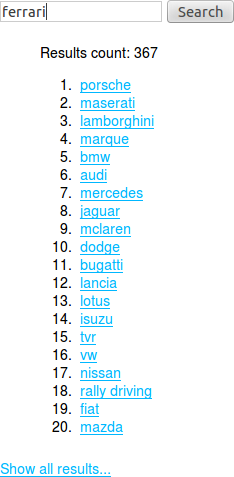
\includegraphics[height=0.6\textwidth]{figures/serelex}
		
\includegraphics[height=0.5\textwidth]{figures/spacer}
		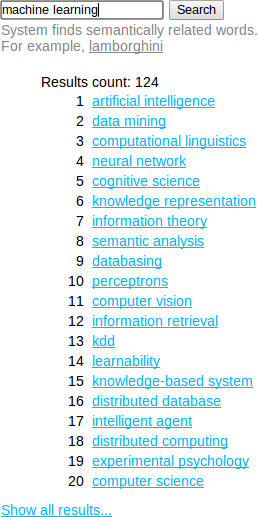
\includegraphics[height=0.6\textwidth]{figures/serelex-ml}
		\end{figure}
\end{itemize}

\end{frame}

\begin{frame}
\frametitle{Try a Demo}

\begin{itemize}
  \item {\bf \url{http://serelex.cental.be/} }
  
\begin{figure}	
	\centering
		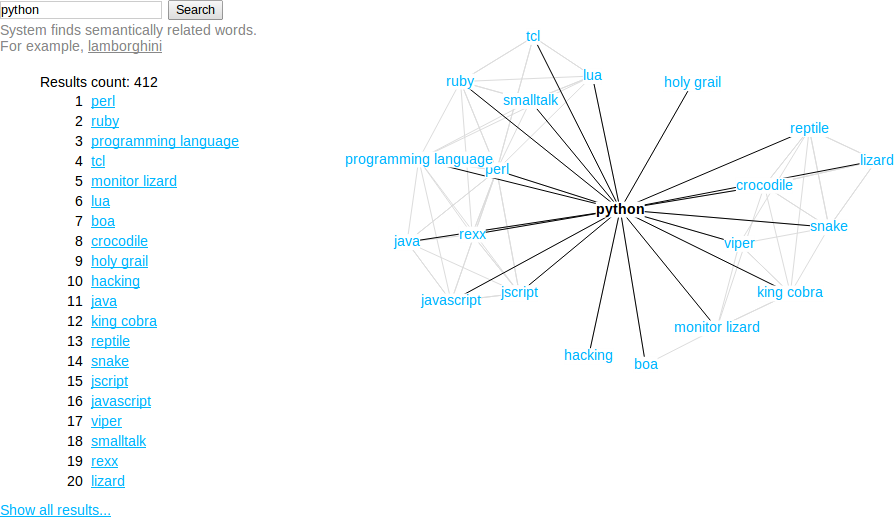
\includegraphics[width=1.0\textwidth]{figures/python}
		\end{figure}
\end{itemize}

\end{frame}

\section{Pattern-Based Similarity Measures}
\subsection{Introduction}

\begin{frame}
\frametitle{Reference Papers}

\begin{itemize}
\item Panchenko A., Morozova O., Naets H. \textbf{“A Semantic Similarity Measure Based on Lexico-Syntactic Patterns''.} In Proceedings of the 11th Conference on Natural Language Processing KONVENS 2012, pp.174--178, Vienna, 2012
\item Panchenko A., Romanov P., Morozova O., Naets H., Philippovich A., Fairon C.. \textbf{Lexico-Semantic Search Engine "Serelex"}. Submitted to the 35th European Conference on Information Retrieval (ECIR 2013).
\end{itemize}
\end{frame}

\subsection{Lexico-Syntactic Patterns}

\begin{frame}
\frametitle{General architecture}

\begin{itemize}
  \item 6 classical Hearst (1992) patterns 
  \item 12 further patterns 
  \item extracting \textbf{hypernyms}, \textbf{co-hyponyms} and \textbf{synonyms}
\begin{figure}	
	\centering
		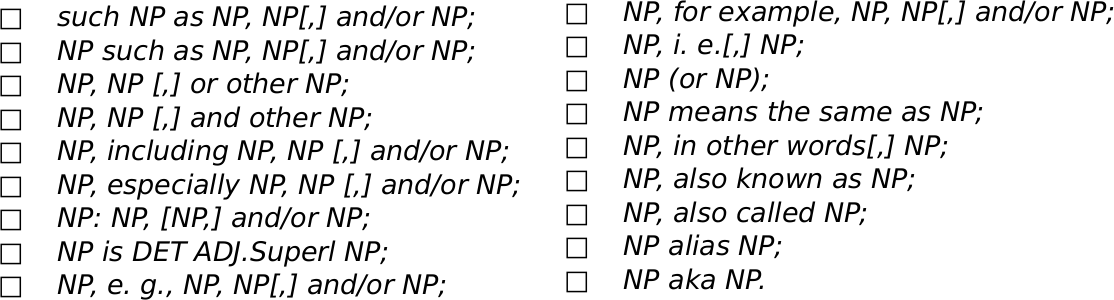
\includegraphics[width=1.0\textwidth]{figures/patterns}
	\end{figure}
\end{itemize}

\end{frame}

\begin{frame}
\frametitle{The main transducer}

\begin{itemize}
  \item A cascade of FSTs
  \item \texttt{Unitex}
\begin{figure}	
	\centering
		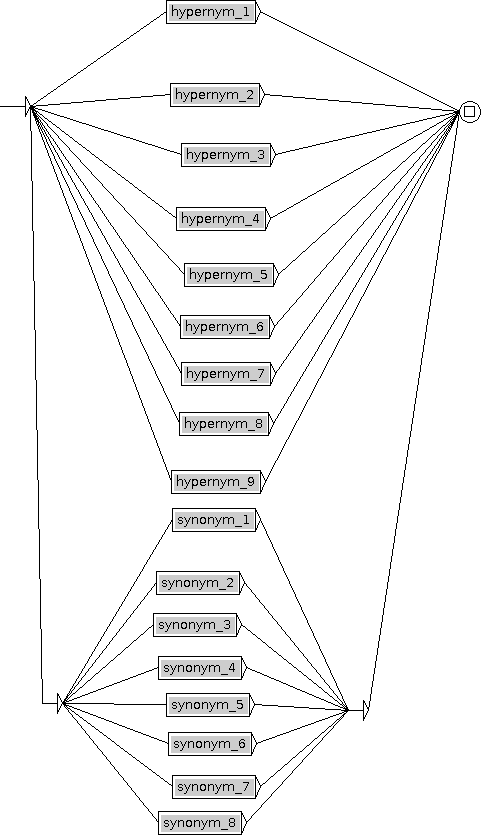
\includegraphics[width=0.3\textwidth]{figures/main-graph}
	\end{figure}
\end{itemize}

\end{frame}


\begin{frame}
\frametitle{The 2nd pattern}

\begin{figure}	
	\centering
		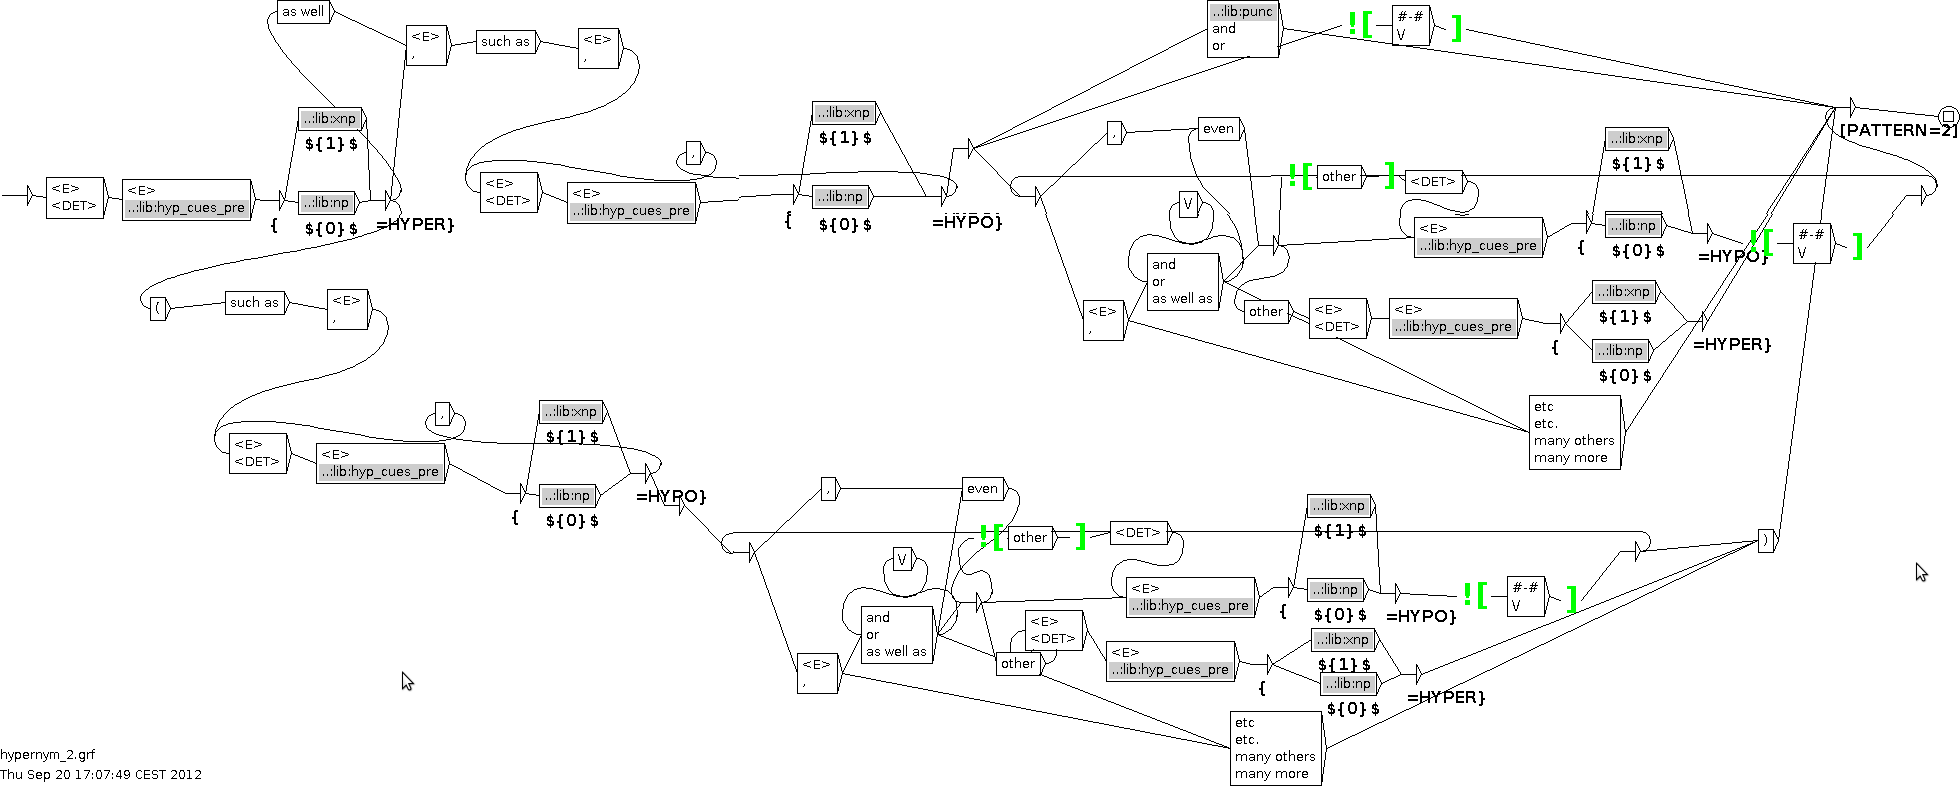
\includegraphics[width=1.0\textwidth]{figures/pattern2}
	\end{figure}

\begin{itemize}
  \item Allow for language variation, preserving precision
	  \item Compare to surface-based patterns (Bollegala et al., 2007)
	
\end{itemize}

\end{frame}


%\begin{frame}
%\frametitle{Explicit extraction rules}

%\begin{itemize}
%	  \item positive/negative contexts,
%	  \item dictionaries,	
%	  \item insertions of adjectives, \ldots
%\end{itemize}

%\begin{figure}	
%	\centering
%		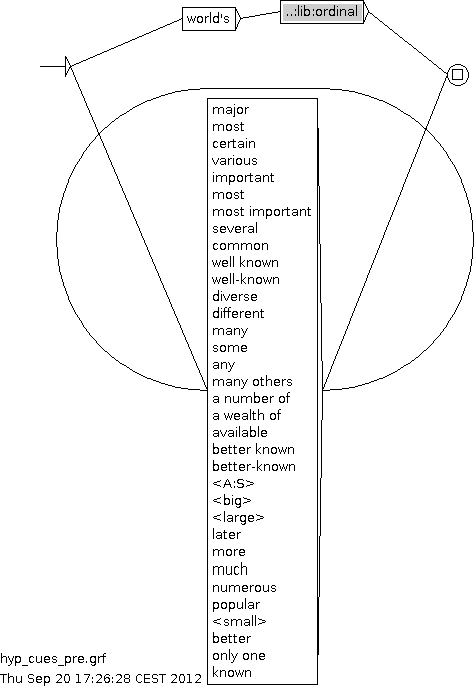
\includegraphics[width=0.3\textwidth]{figures/cues}
%	\end{figure}


%\end{frame}

\begin{frame}
\frametitle{Patterns are applied to texts}

%\begin{figure}	
%	\centering
%		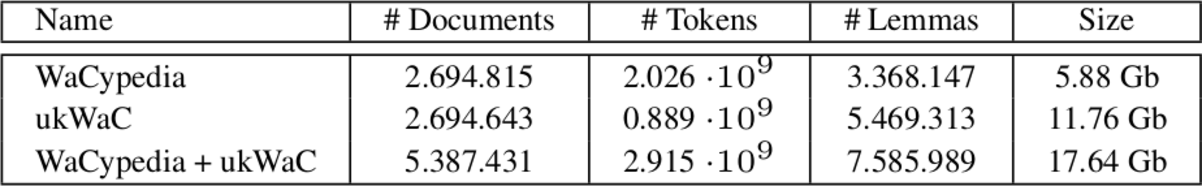
\includegraphics[width=0.9\textwidth]{figures/drawing}
%\end{figure}


\begin{itemize}
  \item \textbf{Wikipedia + ukWaC} 
  \begin{itemize}
    \item 5,387,431 documents
    \item 2.915 $\cdot 10^9$ tokens
    \item 7,585,989 lemmas
    \item 17.65 Gb
  \end{itemize}
	  \item No preprocessing is needed
	  \item 250Mb blocks 
	  \item 1 block $\approx$ 1 hour @ Intel i5 M520@2.40GHz
	  	
\end{itemize}
\end{frame}


\begin{frame}
\frametitle{Patterns extract concordances}

\begin{itemize}
  \item \texttt{such diverse \{[occupations]\} as
  \{[doctors]\}, \{[engineers]\} and \{[scientists]\}[PATTERN=1]}
  \item \texttt{such \{non-alcoholic [sodas]\} as \{[root beer]\} and \{[cream soda]\}[PATTERN=1]}
  \item \texttt{\{traditional[food]\}, such as \{[sandwich]\},\{[burger]\}, and \{[fry]\}[PATTERN=2]}
\end{itemize}

\textbf{Number of concordances:}

\begin{itemize}
  \item Wikipedia -- 1.196.468 
  \item ukWaC -- 2.227.025 
  \item Wikipedia + ukWaC -- 3.423.493
\end{itemize}


\end{frame}

\subsection{Semantic Similarity Measure}

\begin{frame}
\frametitle{General procedure}

\begin{figure}	
	\centering
		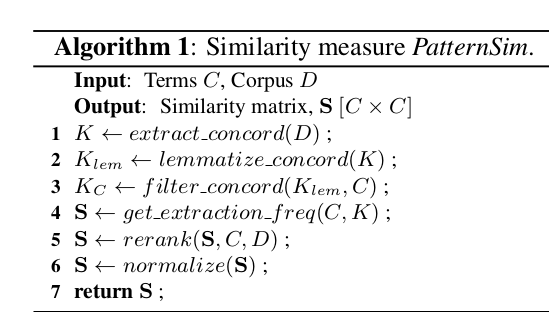
\includegraphics[width=0.65\textwidth]{figures/algo}
\end{figure}

\end{frame}

%\begin{frame}
%\frametitle{Reranking }

%\begin{itemize}

%\item \textbf{Efreq}. No re-ranking. 

%$$s_{ij} = e_{ij}$$

%$s_{ij}$ -- semantic similarity between terms $c_i, c_j \in C$

%$e_{ij}$ --  frequency of co-occurrence of $c_i$ and $c_j$ in concordances $K$ 

%\item \textbf{Efreq-Rfreq}. Penalizes terms strongly related to many words.
%$$
%s_{ij} = \frac{2\cdot\alpha\cdot e_{ij}}{e_{i*} + e_{*j}},
%$$

%$e_{i*}$ -- a number of concordances containing word $c_i$

%$\alpha$ -- an expected number of semantically related words per term 
 
%\end{itemize}

%\end{frame}


%\begin{frame}
%\frametitle{Reranking }

%\begin{itemize}
%\item \textbf{Efreq-Rnum}. Penalizes terms strongly related to many words:

%$$s_{ij} = \frac{2\cdot\mu_b \cdot e_{ij}}{b_{i*} + b_{*j}}, $$


%\item \textbf{Efreq-Cfreq}. Penalizes relations to general words e.g. ``item''. 

%$$s_{ij} = \frac{P(c_i,c_j)}{P(c_i)P(c_j)}$$


 
 
%\end{itemize}

%\end{frame}


\begin{frame}
\frametitle{Reranking formula Efreq-Rnum-Cfreq-Pnum}

  
$$s_{ij} = \sqrt{p_{ij}} \cdot \frac{2\cdot\mu_b }{b_{i*}+b_{*j}} \cdot \frac{P(c_i,c_j)}{P(c_i)P(c_j)}.$$


\begin{itemize}

%\item $s_{ij}$ -- semantic similarity between terms $c_i, c_j \in C$

\item $P(c_i,c_j)=\frac{e_{ij}}{\sum_{ij}e_{ij}}$ -- extraction probability of the pair $\langle c_i,c_j \rangle$, $e_{ij}$ --  frequency of co-occurrence of $c_i$ and $c_j$ in concordances $K$ 

\item $P(c_i)= \frac{f_i}{\sum_i f_i}$ -- probability of the term $c_i$, $f_i$ -- frequency of $c_i$ 
\item $b_{i*} = \sum_{j:e_{ij} \geq \beta} 1$ -- the number of extractions for term $c_i$ with the frequency $\geq \beta$, $\mu_b = \frac{1}{|C|}\sum_{i=1}^{|C|} b_{i*}$ -- the average number of extractions per term

\item $p_{ij} \in [1;18]$ -- number of distinct patterns extracted the relation $\langle c_i, c_j \rangle$
  
 
\end{itemize}

\end{frame}





\subsection{Results}

%%%%%%%%%%%%%%%%%%%%%%%%%%%%%%%%%%%%%%%%%%%%%%%%%
\begin{frame}
\frametitle{Correlation with Human Judgements}

\begin{table}[h]\footnotesize
\begin{tabular}{ |c|c|c|c|c|c| }
\hline
  term, $c_i$ & term, $c_j$ & judgement, $\mathbf{s}$  & sim, $\mathbf{s}$  & judgement, $\mathbf{r}$ & sim, $\hat{\mathbf{r}}$  \\ \hline \hline
tiger & cat & 7.35 & 0.85 & 1 & 3 \\
book & paper & 7.46 &  0.95 & 2 & 2 \\
computer & keyboard & 7.62 &  0.81 & 3 & 1 \\
... & ... & ... & ...   & \ldots & \ldots \\
possibility & girl & 1.94 & 0.25 & 64 & 65 \\
sugar & approach & 0.88 & 0.05 & 65 & 23 \\ \hline
\end{tabular}
\end{table}


\textbf{Data:}

\begin{itemize}
	\item WordSim353 -- 353 term pairs (Finkelstein, 2002)  
	\item MC -- 30 term pairs  (Miller & Charles, 1991)
	\item RG -- 65 term pairs (Rubenstein & Goodenough, 1965)  
\end{itemize}

\textbf{Criteria:}
\begin{itemize}
\item Pearson correlation:  $\rho = \frac{cov(\mathbf{s},\hat{\mathbf{s}})}{\sigma(\mathbf{s}) \sigma(\hat{\mathbf{s}})}$

 \item Spearman's correlation: $r = \frac{cov(\mathbf{r},\hat{\mathbf{r}})}{\sigma(\mathbf{r}) \sigma(\hat{\mathbf{r}})}$
 
 \end{itemize}
 
\end{frame}

\begin{frame}
\frametitle{Correlation with Human Judgements}

\begin{figure}	
	\centering
	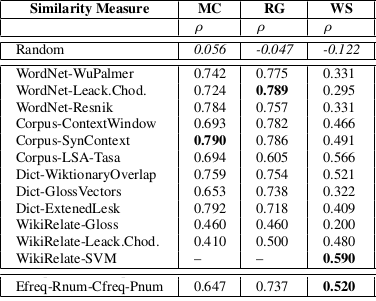
\includegraphics[width=0.5\textwidth]{figures/res-hj-mlg}
\end{figure}

\end{frame}


\begin{frame}
\frametitle{Semantic Relation Ranking}

{ \scriptsize

\begin{table}[h]\footnotesize
\begin{tabular}{ |c|l|l| }
\hline
term, $c_i$ & term, $c_j$ & relation type, $t$  \\ \hline \hline
judge & adjudicate & syn \\
judge & arbitrate & syn \\
%judge & asessor & syn \\
judge & chancellor & syn \\
%judge & gendarmerie & syn \\
... & ... & ...   \\
judge & pc & random \\ 
judge & fare & random \\
judge & lemon & random \\ \hline
\end{tabular}
\end {table}

}

\begin{itemize}
  \item \textbf{BLESS} (Baroni and Lenci, 2011)
  \begin{itemize}
    \item 26,554 relations
    \item hyperonyms, co-hypernyms, meronyms, associations, attributes, random relations
    \end{itemize}  
  \item \textbf{SN} (Panchenko and Morozova, 2012)
  \begin{itemize}
    \item 14,682  relations\
    \item synonyms, co-hyponyms, hyponyms, random relations
    \end{itemize}
    
    %\item $\frac{|R_{random}|}{|R|} \approx 0.5$
     
\end{itemize}

\end{frame}

%%%%%%%%%%%%%%%%%%%%%%%%%%%%%%%%%%%%%%%%%%%%%%%%%
\begin{frame}
\frametitle{Semantic Relation Ranking}

\begin{itemize}
  
  \item Based on the number of correctly ranked relations.

\item $R$ -- all non-random relations 

\item $\hat{R}(k)$ --  top k\% relations of targets


\begin{block}{Criteria}

	
	\begin{itemize}
		\item Precision: $P(k)=$$\frac{|R \cap \hat{R}(k)|}{|\hat{R}(k)|}$,
		\item Recall: $R(k)=$$\frac{|R \cap \hat{R}(k)|}{|R|}$,
		%\item F1-measure: $F(k)= 2 \cdot \frac{P(k) \cdot R(k)}{P(k) + R(k)}$,
	\end{itemize}	
	\end{block}

\item We use $P(10)$, $P(20)$, $P(50)$, $R(50)$.
	

\end{itemize}
	
	
\end{frame}


%%%%%%%%%%%%%%%%%%%%%%%%%%%%%%%%%%%%%%%%%%%%%%%%%
\begin{frame}
\frametitle{Semantic Relation Ranking}

\begin{itemize}
	\item Precision $P(50\%)= \frac{1}{7} \approx 0.86 $
\end{itemize}

\begin{table}[h]\footnotesize
\begin{tabular}{ |l|l|l|l| }
\hline
 term, $c_i$ &  term, $c_j$ & relation type & \bf $s_{ij}$ \\ \hline \hline

aficionado & enthusiast & syn & 0.07197 \\
aficionado & fan & syn & 0.05195 \\
aficionado & admirer & syn & 0.01964 \\
aficionado & addict & syn & 0.01326 \\
aficionado & devotee & syn & 0.01163 \\
aficionado & foundling & random & 0.00777 \\
aficionado & fanatic & syn & 0.00414 \\ \hline
aficionado & adherent & syn & 0.00353 \\
aficionado & capital & random & 0.00232 \\
aficionado & statute & random & 0.00029 \\
aficionado & blot & random & 0.00025 \\
aficionado & meddler & random & 0.00005 \\
aficionado & enlargement & random &	0.00003 \\
aficionado & bawdyhouse & random & 	0.00000 \\ 
\hline
\end{tabular}
\end {table}

\end{frame}

\begin{frame}
\frametitle{Semantic Relation Ranking}

\begin{figure}	
	\centering
	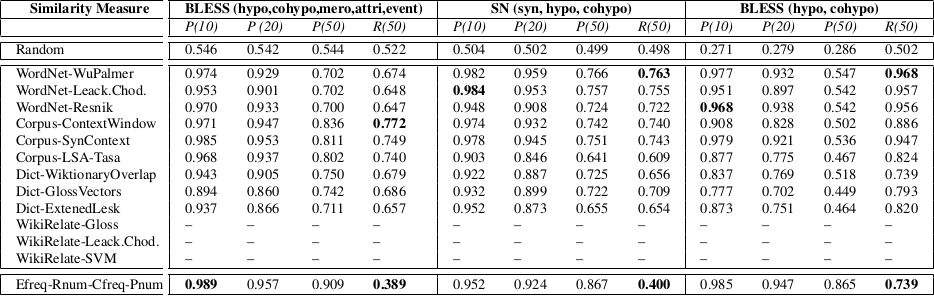
\includegraphics[width=1.0\textwidth]{figures/res-relations-mlg}
\end{figure}

\end{frame}


\begin{frame}
\frametitle{Semantic Relation Ranking}

\begin{figure}	
	\centering
	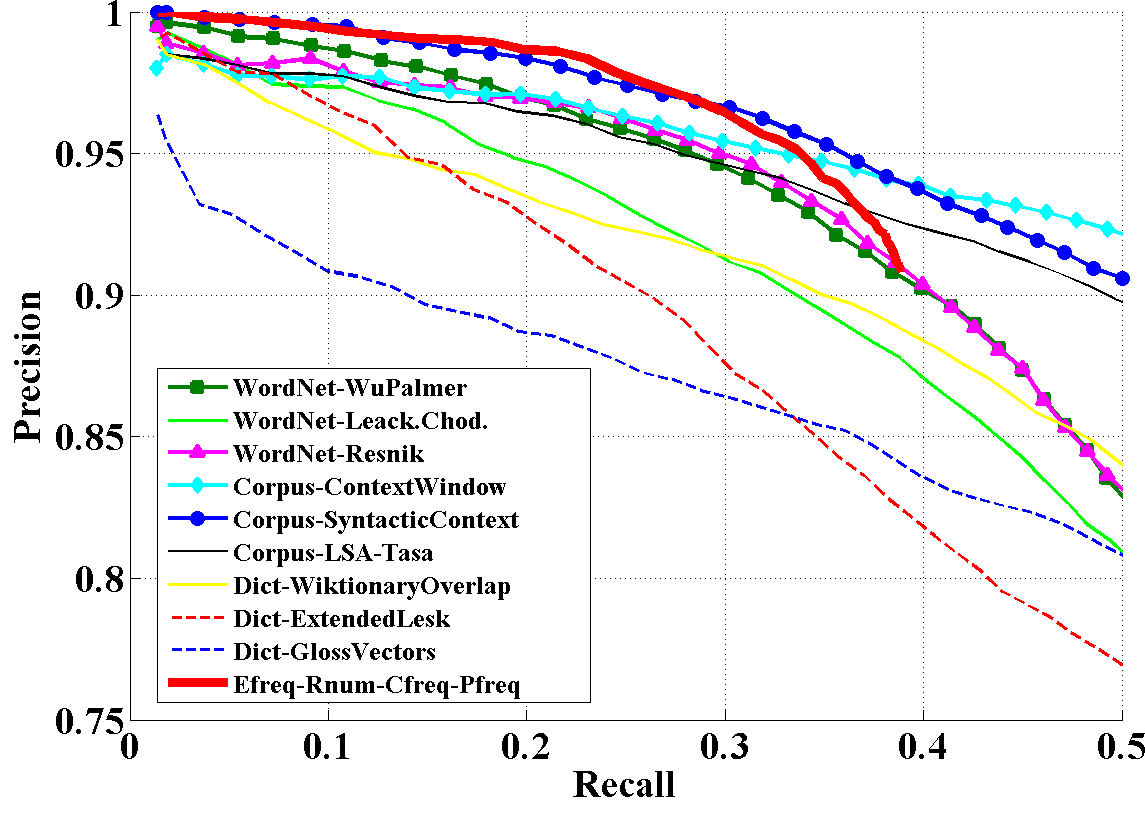
\includegraphics[width=0.7\textwidth]{figures/pr2-mlg}
	\caption{Precision-Recall graphs calculated on the BLESS dataset: the pattern-based measure versus the baselines.
	}
\end{figure}

\end{frame}

\begin{frame}
\frametitle{Semantic Relation Extraction}

\begin{figure}	
	\centering
	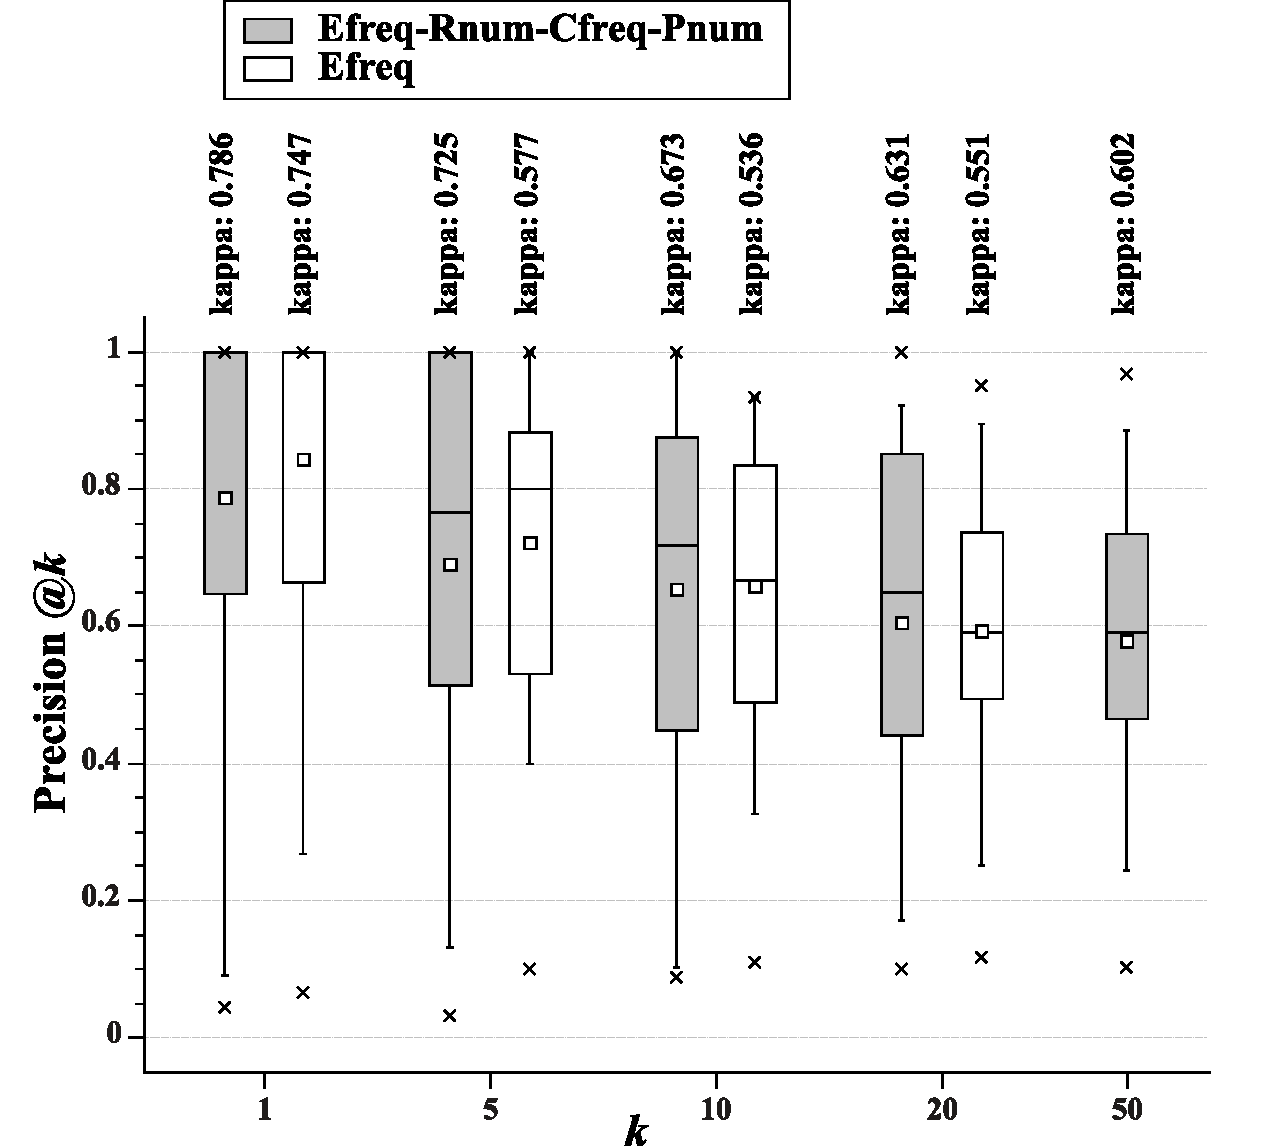
\includegraphics[width=0.5\textwidth]{figures/b}
	\caption{Semantic relation extraction: precision at k.}
\end{figure}

\begin{itemize}
  \item 49 words  -- vocabulary of the RG dataset
  \item three annotators, binary annotations  
\end{itemize}

\end{frame}



\subsection{Conclusion}


\begin{frame}
\frametitle{Conclusion}

\begin{itemize}
  \item We presented a similarity measure based on \textbf{manually-crafted lexico-syntactic patterns}.
 

\item The measure provides results \textbf{comparable to the baselines} and \textbf{does not require semantic resources}.

\item Future work -- using \textbf{a supervised model} to
\begin{itemize}
\item combine different factors of Efreq-Rnum-Cfreq-Pnum;
\item tune the meta-parameters of Efreq-Rnum-Cfreq-Pnum.
\end{itemize}
    
\end{itemize}

%\textbf{Data:} {\footnotesize \url{http://cental.fltr.ucl.ac.be/team/~panchenko/sim-eval/ } }

\textbf{Code:} {\footnotesize \url{http://github.com/cental/patternsim/}}

\textbf{Demo:} {\footnotesize \url{http://serelex.cental.be/}}


\end{frame}



%%%%%%%%%%%%%%%%%%%%%%%%%%%%%%%%%%%%%%%%%%%%%%%%%
\section{Hybrid Semantic Similarity Measures}

\subsection{Introduction}

%%%%%%%%%%%%%%%%%%%%%%%%%%%%%%%%%%%%%%%%%%%%%%%%%%


\begin{frame}
\frametitle{Reference Paper}

\begin{itemize}

\item Panchenko A. Morozova O. \textbf{“A Study of Hybrid Similarity Measures for Semantic Relation Extraction”}. In Proceedings of Workshop of Innovative Hybrid Approaches to the Processing of Textual Data Workshop, EACL 2012, pp.10-18, 2012
\end{itemize}

\end{frame}


\begin{frame}
\frametitle{The State of Art}
\begin{itemize}
\item A multitude of \textbf{complimentary measures} were proposed to extract synonyms, hypernyms,
and co-hyponyms

\item Most of them are based on \textbf{one} of the \textbf{5 key approaches}: 
\begin{enumerate}
\item distributional analysis (Lin, 1998b)
\item web as a corpus (Cilibrasi and Vitanyi, 2007)
\item lexico-syntactic patterns (Bollegala et al., 2007)
\item semantic networks (Resnik, 1995)
\item definitions of dictionaries or encyclopedias (Zesch et al., 2008a)
\end{enumerate}


\item Some attempts were made to \textbf{combine measures} (Curran, 2002; Cederberg and Widdows, 2003; Mihalcea et al., 2006;
Agirre et al., 2009; Yang and Callan, 2009)


\item However, most studies are still \textbf{not taking into account}
all 5 existing extraction approaches.

\end{itemize}
%\textbf{Research Question}: How to combine the baseline similarity measures to improve relation extraction? 

\end{frame}


%%%%%%%%%%%%%%%%%%%%%%%%%%%%%%%%%%%%%%%%%%%%%%%%%%
%\begin{frame}
%\frametitle{Contributions}
%\begin{itemize}
%\item A systematic analysis of 
%\begin{itemize}
%  \item \textbf{16 baseline similarity measures} of 5 key extraction principles
%  \item their combinations with \textbf{8 fusion methods} 
%\end{itemize}

%\item \textbf{Hybrid similarity measures} based on all the 5 extraction approaches:
%\begin{enumerate}
%  \item distributional analysis
%  \item Web as a corpus 
%  \item	lexico-syntactic patterns
%  \item	semantic networks 
%  \item definitions of dictionaries or encyclopedias 
%\end{enumerate}

%\item The best found hybrid measure combines 15 baseline measures with the Logistic Regression
 

%\end{itemize}

%\end{frame}


\begin{frame}
\frametitle{Single and Hybrid Similarity Measures}
\begin{itemize}
\item 16 \textbf{single} measures
	\begin{itemize}
	\item 5 measures based on a \textbf{semantic network} 
	\item 3 \textbf{web-based} measures
	\item 5 \textbf{corpus-based} measures 
	\begin{itemize}
	  \item 2 distributional
	  \item 1 lexico-syntactic patterns
	  \item 2 other co-occurence based
	\end{itemize}
	\item 3 \textbf{definition-based} measures 
\end{itemize}
\item 64 \textbf{hybrid} measures
	\begin{itemize}
	\item 8 \textbf{combination methods}
	\item 8 \textbf{measure sets} obtained with 3 measure selection techniques
	\end{itemize}
\end{itemize}

\end{frame}

\subsection{Features: Single Similarity Measures}

%%%%%%%%%%%%%%%%%%%%%%%%%%%%%%%%%%%%%%%%%%%%%%%%%
\begin{frame}
\frametitle{Measures Based on a Semantic Network}

\begin{enumerate}
  \item Wu and Palmer (1994)
 \item Leacock and Chodorow (1998)
 \item Resnik (1995)
 \item Jiang and Conrath (1997)
 \item Lin (1998)
\end{enumerate}


 \textbf{Data:} 
 \begin{itemize}
   \item WordNet 3.0
   \item SemCor corpus
	
 \end{itemize}
 \textbf{Variables:}
 \begin{itemize}
  \item Lengths of the shortest paths between terms in the network
 \item Probability of terms derived from a corpus
 \end{itemize}
 
 \textbf{Coverage:} 155.287 English terms encoded in WordNet 3.0.
 
\end{frame}

%%%%%%%%%%%%%%%%%%%%%%%%%%%%%%%%%%%%%%%%%%%%%%%%%
\begin{frame}
\frametitle{Web-based Measures}
	
Normalized Google Distance (NGD) (Cilibrasi and Vitanyi, 2007)

\begin{enumerate}
   \setcounter{enumi}{5}
   \item NGD-Yahoo! 
   \item NGD-Bing 
   \item NGD-Google over wikipedia.org domain     
\end{enumerate}

\textbf{Data:} number of times the terms co-occur in the documents
as indexed by an IR system.

\textbf{Variables:} 

\begin{itemize}
	\item \textbf{number of hits} returned by query $"c_i"$ 
	\item \textbf{number of hits} returned by query $"c_i \text{ AND } c_j''$
\end{itemize}

\textbf{Coverage:} huge vocabulary in dozens of languages.


\end{frame}

%%%%%%%%%%%%%%%%%%%%%%%%%%%%%%%%%%%%%%%%%%%%%%%%%
\begin{frame}
\frametitle{Corpus-based Measures}

\begin{enumerate}
   \setcounter{enumi}{8}
	\item Bag-of-word Distributional Analysis (BDA) (Sahlgren, 2006) 
	\item Syntactic Distributional Analysis (SDA) (Curran, 2003) 
\end{enumerate}

\textbf{Data:} WaCkypedia (800M tokens) and PukWaC (2000M tokens) corpora (Baroni et al., 2009) 
 
\textbf{Variables:} 
\begin{itemize}
  \item feature vector based on the \textbf{context window}
  \item feature vector based on the \textbf{syntactic context} 
\end{itemize}

\textbf{Coverage:} word should occur in the corpora.
	
\end{frame}

%%%%%%%%%%%%%%%%%%%%%%%%%%%%%%%%%%%%%%%%%%%%%%%%%
%\begin{frame}
%\frametitle{Corpus-based Measures }

%\begin{enumerate}
%  \setcounter{enumi}{10}
%  \item A measure based on \textbf{lexico-syntactic patterns}   
%\end{enumerate}	
 
%\textbf{Data}: WaCkypedia corpus (800M tokens) 

%\textbf{Method:}
%\begin{itemize}
%  \item A pattern-based measure as presented before. 
	%\item 10 patterns for hypernymy extraction: 6 Hearst (1992) patterns + 4 other patterns
	
	%\item \texttt{such diverse \{[occupations]\} as
  %\{[doctors]\}, \{[engineers]\} and \{[scientists]\}[PATTERN=1]}
  
  %\item \textbf{Efreq}: semantic similarity $s_{ij}$ between terms $c_i, c_j \in C$ -- 
 %the number of term co-occurences in the same concordance $n_{ij}$:
  
   %$$
   %sim(c_i,c_j) = s_{ij} = \frac{n_{ij}}{max_{ij}(n_{ij})}.
   %$$
%\end{itemize}
 
% \end{frame}
 
%\begin{frame}


%\frametitle{Corpus-based Measures}
	
% \begin{figure}
 %       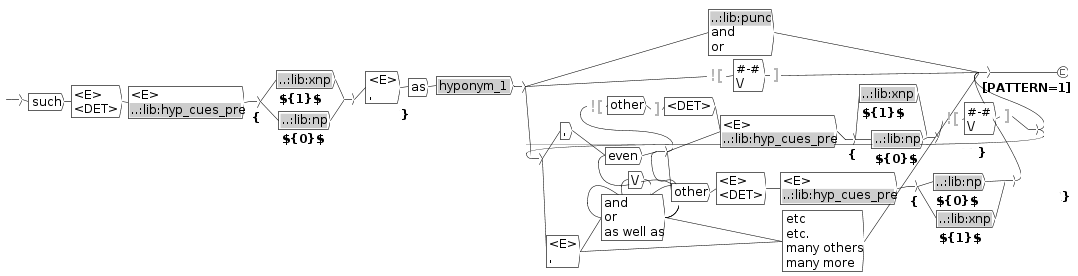
\includegraphics[width=1.0\textwidth]{figures/hypernym_1}
  %      \caption{A UNITEX graph implementing the first extraction pattern.}
   %     \label{fig:prcomb}
%\end{figure}

%\textbf{Coverage:} Target terms $c_i, c_j$ should co-occur in a sentence.
	
%\end{frame}

\begin{frame}
\frametitle{Corpus-based Measures }

\begin{enumerate}
   \setcounter{enumi}{10}
   \item \textbf{PatternSim}, presented before;
	\item \textbf{Latent Semantic Analysis (LSA)} on TASA corpus (Landauer and Dumais, 1997);
	\item \textbf{NGD} on Factiva corpus (Veksler et al., 2008).
\end{enumerate}
	
\end{frame}

%%%%%%%%%%%%%%%%%%%%%%%%%%%%%%%%%%%%%%%%%%%%%%%%%
\begin{frame}
\frametitle{Definition-based Measures}

\begin{enumerate}
  \setcounter{enumi}{13}
  \item \textbf{Extended Lesk}  (Banerjee and Pedersen, 2003)
  \item \textbf{GlossVectors} (Patwardhan and Pedersen, 2006)
\end{enumerate}


\textbf{Data:} WordNet glosses.
	
\textbf{Variables:}
\begin{itemize}
		\item bag-of-words vector of a term $c_i$ derived from the glosses
		\item relation  between words $(c_i,c_j)$ in the network 
\end{itemize}

\textbf{Coverage:} 117.659 glosses encoded in WordNet 3.0

\end{frame}


%%%%%%%%%%%%%%%%%%%%%%%%%%%%%%%%%%%%%%%%%%%%%%%%%
\begin{frame}
\frametitle{Definition-based Measures}

\begin{enumerate}
 \setcounter{enumi}{15} 
\item \textbf{WktWiki} -- BDA on definitions of Wiktionary and Wikipedia%~\footnote{The method stems from the work of Zesch et al. (2008)}

\end{enumerate}

\textbf{Data}: Wikipedia abstracts, Wiktionary.

\textbf{Method:}
\begin{itemize}
  \item Definition = abstract of Wikipedia article with title $"c_i"$ + 
   glosses, examples, quotations, related words, categories from Wiktionary  for $c_i$
   \item Represent a definition as a bag-of-words vector
   \item Calculate similarities with cosine
   \item Update similarities according to relations in the Wiktionary.
  
\end{itemize}
   \textbf{Coverage:} Wiktionary: 536.594 glosses, Wikipedia: 3.8M articles
   
\end{frame}


\subsection{Hybrid Similarity Measures}

%%%%%%%%%%%%%%%%%%%%%%%%%%%%%%%%%%%%%%%%%%%%%%%%%
\begin{frame}
\frametitle{Combination Methods}
\begin{itemize}
\item A \textbf{goal of a combination method} is to produce ``better'' similarity scores than the
scores of single measures.

\item A \textbf{combination method} takes as an input   
$\{\mathbf{S}_1,\ldots,\mathbf{S}_K\}$ produced by $K$ single measures and
outputs  $\mathbf{S}_{cmb}$.

\item $s_{ij}^k \in \mathbf{S}_k$ is a \textbf{pairwise similarity score} of terms $c_i$ and $c_j$ produced by $k$-th measure.

\item We tested \textbf{8  combination methods}.

\end{itemize}
\end{frame}

\begin{frame}
\frametitle{Unsupervised Combination Methods}

\begin{enumerate}
  
\item \textbf{Mean}. A mean of $K$ pairwise similarity scores:

$$\mathbf{S}_{cmb} = \frac{1}{K} \sum_{k=1}^K \mathbf{S}_k \Leftrightarrow 
s_{ij}^{cmb}= \frac{1}{K}\sum_{k=1,K} s_{ij}^k.$$

\item \textbf{Mean-Nnz}. A mean of scores having non-zero value:
 $$s_{ij}^{cmb}= \frac{1}{|k:s_{ij}^k
>0,k=1,K|}\sum_{k=1,K} s_{ij}^k.$$

\item \textbf{Mean-Zscore}. A mean of scores
transformed into Z-scores:
$$\mathbf{S}_{cmb} = \frac{1}{K} \sum_{k=1}^K \frac{\mathbf{S}_k -
\mu_k}{\sigma_k},$$ where $\mu_k$ and $\sigma_k$ are a mean and a standard deviation of the scores of the $k$-th measure ($\mathbf{S}_k$).

\end{enumerate}
\end{frame}



\begin{frame}
\frametitle{Unsupervised Combination Methods}

\begin{enumerate}
  \setcounter{enumi}{3}
\item \textbf{Median}. A median of $K$ pairwise similarities:
$$s_{ij}^{cmb}= median(s_{ij}^1,\ldots,s_{ij}^K). $$

\item \textbf{Max}. A maximum of $K$ pairwise similarities:
$$s_{ij}^{cmb}= max(s_{ij}^1,\ldots,s_{ij}^K).$$

\item \textbf{RankFusion}. A mean of scores converted to ranks:
 $$s_{ij}^{cmb}= \frac{1}{K}\sum_{k=1,K}
r_{ij}^k,$$
where  $r^k_{ij}$ is the rank corresponding to the similarity score $s^k_{ij}$.
\item \textbf{RelationFusion} (Panchenko and Morozova, 2012).
\end{enumerate}

\end{frame}



%\begin{frame}
%\frametitle{Combination Methods}

%\begin{enumerate}
%  \setcounter{enumi}{6}
%  \item \textbf{RelationFusion}. 
%  \begin{itemize}
%  \item Unions the top relations found by each measure separately.
%  \item A relation extracted by several measures has more weight.
%  \item See (Panchenko and Morozova, 2012) for details. 
%\end{itemize}
%\begin{algorithm}[H]
%\SetLine
%\KwIn{Similarity matrices of $N$ single measures $\{\mathbf{S}_1,\ldots,\mathbf{S}_N\}$, number of nearest neighbors $K$}
%\KwOut{ Combined similarity matrix $\mathbf{S}_{cmb}$  }

%\For{i=1,N}{
%	$R_i = knn(\mathbf{S}_i, k)$ \;
% 	$\mathbf{R}_i = relation\_matrix(R_i)$
% }
%$\mathbf{S}_{cmb} = \frac{1}{N} \sum_{i=1}^N \mathbf{R}_i$ \;
%\Return $\mathbf{S}_{cmb}$ \;
%\label{rfusion}
%\end{algorithm}
%$$
%r^k_{ij} \in \mathbf{R}_k, r_{ij}^k = \left\{ 
%  \begin{array}{l l}
%    1 & \quad \text{if relation } \langle c_i, c_j \rangle \in R_k \\
%    0 & \quad \text{else}\\
%  \end{array} \right.
%$$

%\end{enumerate}

%\end{frame}

\begin{frame}
\frametitle{Supervised Combination Methods}

\begin{enumerate}
  \setcounter{enumi}{7}
\item \textbf{Logit}. 

\begin{itemize}
  \item  Training a \textbf{binary classifier} (a Logistic Regression) on a set of manually constructed
semantic relations $R$ (BLESS or SN)

\item \textbf{Positive training examples} are “meaningful” relations (synonyms,
hyponyms, co-hyponyms, associations)
\item \textbf{Negative training examples} are pairs of semantically unrelated words (generated randomly and verified manually).


  \item A relation $\langle c_i,t, c_j \rangle \in R$ is represented with an $N$-dimensional \textbf{vector of pairwise similarities}: $\mathbf{x}_{ij} = (s_{ij}^1,\ldots,s_{ij}^N)$. 

\item Category $y_{ij}$:
$$
y_{ij} = \left\{ 
  \begin{array}{l l}
    0 & \quad  \text{ if } \langle c_i,t, c_j \rangle \text{ is a random relation} 
    \\
    1 & \quad  \text{ otherwise }\\
  \end{array} \right
  .
$$

\item \textbf{Using the model} $(w_1,\ldots,w_K)$ to combine measures: 
$$s^{cmb}_{ij} = \frac{1}{1 + e^{-z}}, z = w_0 + \sum_{k=1}^K w_k s^k_{ij} , $$

\end{itemize}
\end{enumerate}

\end{frame}

%%%%%%%%%%%%%%%%%%%%%%%%%%%%%%%%%%%%%%%%%%%%%%%%%
\begin{frame}
\frametitle{Measure Selection}

\begin{block}{A problem}
 Number of ways to choose which of 16 single measures to combine:

$$ 2^{16}=65.535$$
 
\end{block}


\begin{itemize}
 
\item \textbf{Expert choice of measures} -- 5, 9 and 15 measures
\item \textbf{Forward Stepwise Procedure} -- 7, 8a, 8b, 10 measures 
\item \textbf{Analysis of LR weights} -- 12 measures

\pause

\item The \alert{best predictors}: C-BDA, C-SDA, C-LSA-Tasa, D-WktWiki, D-GlossVectors,  D-ExtendedLesk.

%\begin{itemize}
 %\item \textbf{5} % = WN-Resnik, BDA-3-5000, SDA-21-100000,  Def-WktWiki-1000
 %\item \textbf{9} %= \textbf{Group4} + WN-WuPalmer, LSA-Tasa, Def-GlossVec., and Def-Ext.Les
 %\item \textbf{15} %= \textbf{Group8} + WN-LeacockChodorow, WN-Lin, WN-JiangConrath, NGD-Factiva, NGD-Yahoo, and NGD-GoogleWiki.
%\end{itemize}

\end{itemize}
\end{frame}
  

%%%%%%%%%%%%%%%%%%%%%%%%%%%%%%%%%%%%%%%%%%%%%%%%%

\subsection{Results}
%\subsection{}

%%%%%%%%%%%%%%%%%%%%%%%%%%%%%%%%%%%%%%%%%%%%%%%%%

%\begin{frame}
%\frametitle{Single Similarity Measures}
%	\begin{figure}
%	\centering
%		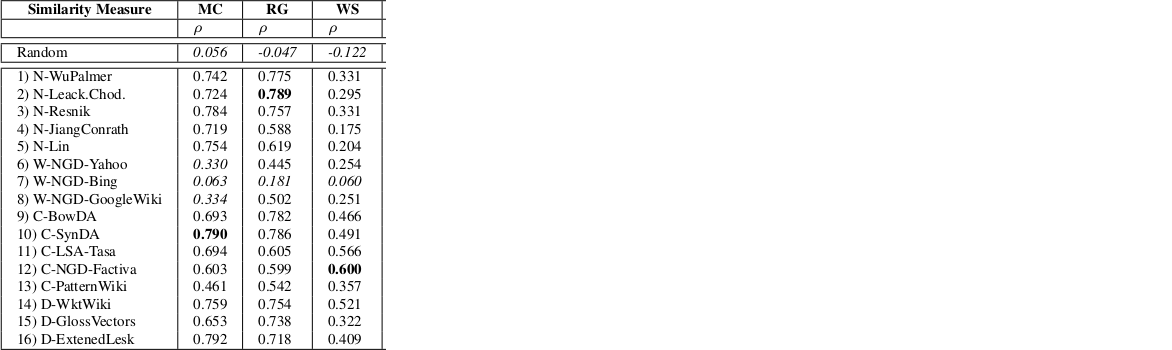
\includegraphics[width=1.0\textwidth]{figures/table-hybrid-single-hg}
%		
%		\caption{ Performance of \textbf{16 single similarity measures} on \textbf{human judgement datasets} (MC, RG,
%WordSim353). The best scores in a group are in
%bold. 
%}
%\end{figure}
	
%\end{frame}


%\begin{frame}
%\frametitle{Single Similarity Measures}
%	\begin{figure}
%	\centering
%		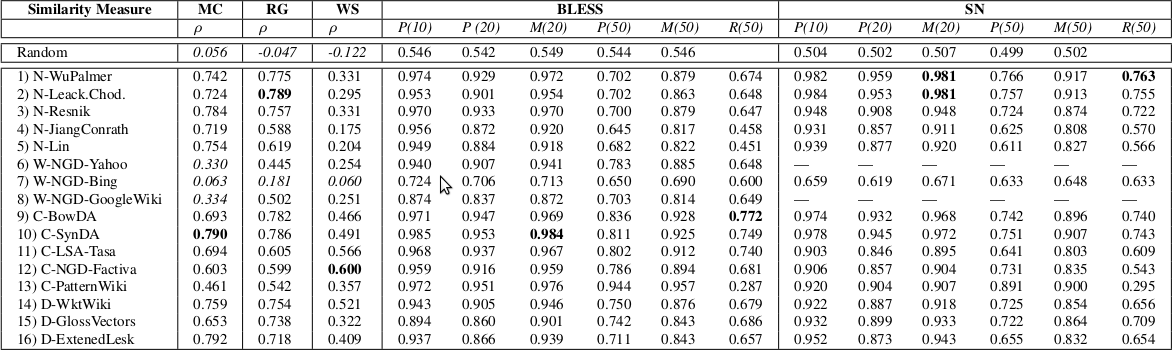
\includegraphics[width=1.0\textwidth]{figures/table-hybrid-single}
%		
%		\caption{ Performance of \textbf{16 single similarity measures} on human judgement datasets (MC, RG,
%WordSim353) and semantic relation datasets (BLESS and SN). The best scores in a group are in
%bold. 
%}
%\end{figure}
	
%\end{frame}

%%%%%%%%%%%%%%%%%%%%%%%%%%%%%%%%%%%%%%%%%%%%%%%%%
\begin{frame}
\frametitle{Hybrid Similarity Measures}

	\begin{figure}
	\centering
		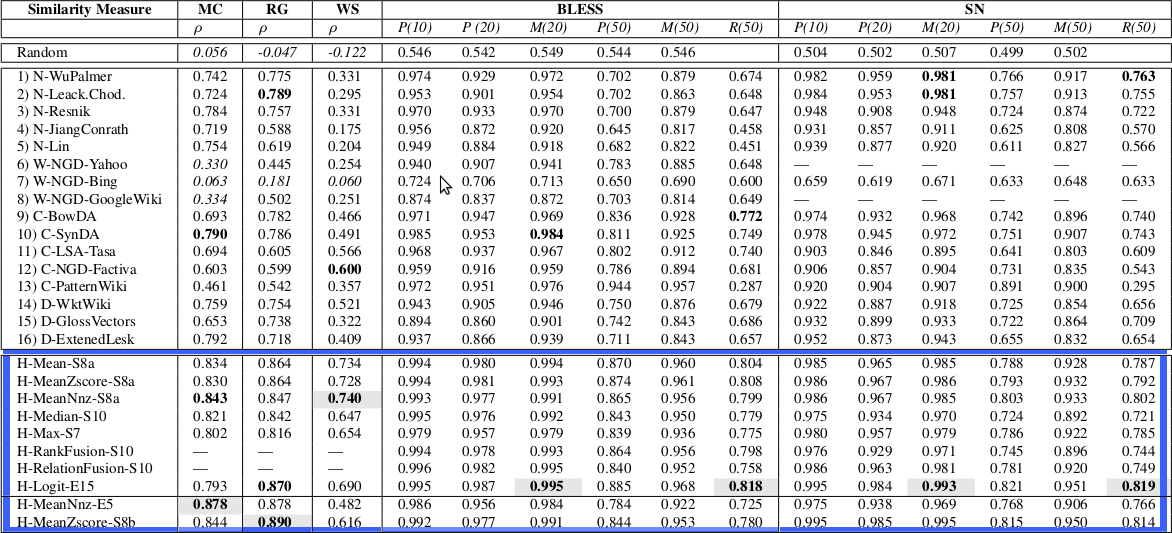
\includegraphics[width=1.0\textwidth]{figures/table-hybrid-hybrid}
		
		\caption{ Performance of \textbf{16 single and 8 hybrid similarity measures} on human judgements datasets (MC, RG,
WordSim353) and semantic relation datasets (BLESS and SN). The best scores in a group (single/hybrid) are in
bold; the very best scores are in grey. }
\end{figure}
	
	
\end{frame}

%%%%%%%%%%%%%%%%%%%%%%%%%%%%%%%%%%%%%%%%%%%%%%%%%
\begin{frame}
 \frametitle{Hybrid Similarity Measures}
	\begin{figure}
	\centering
		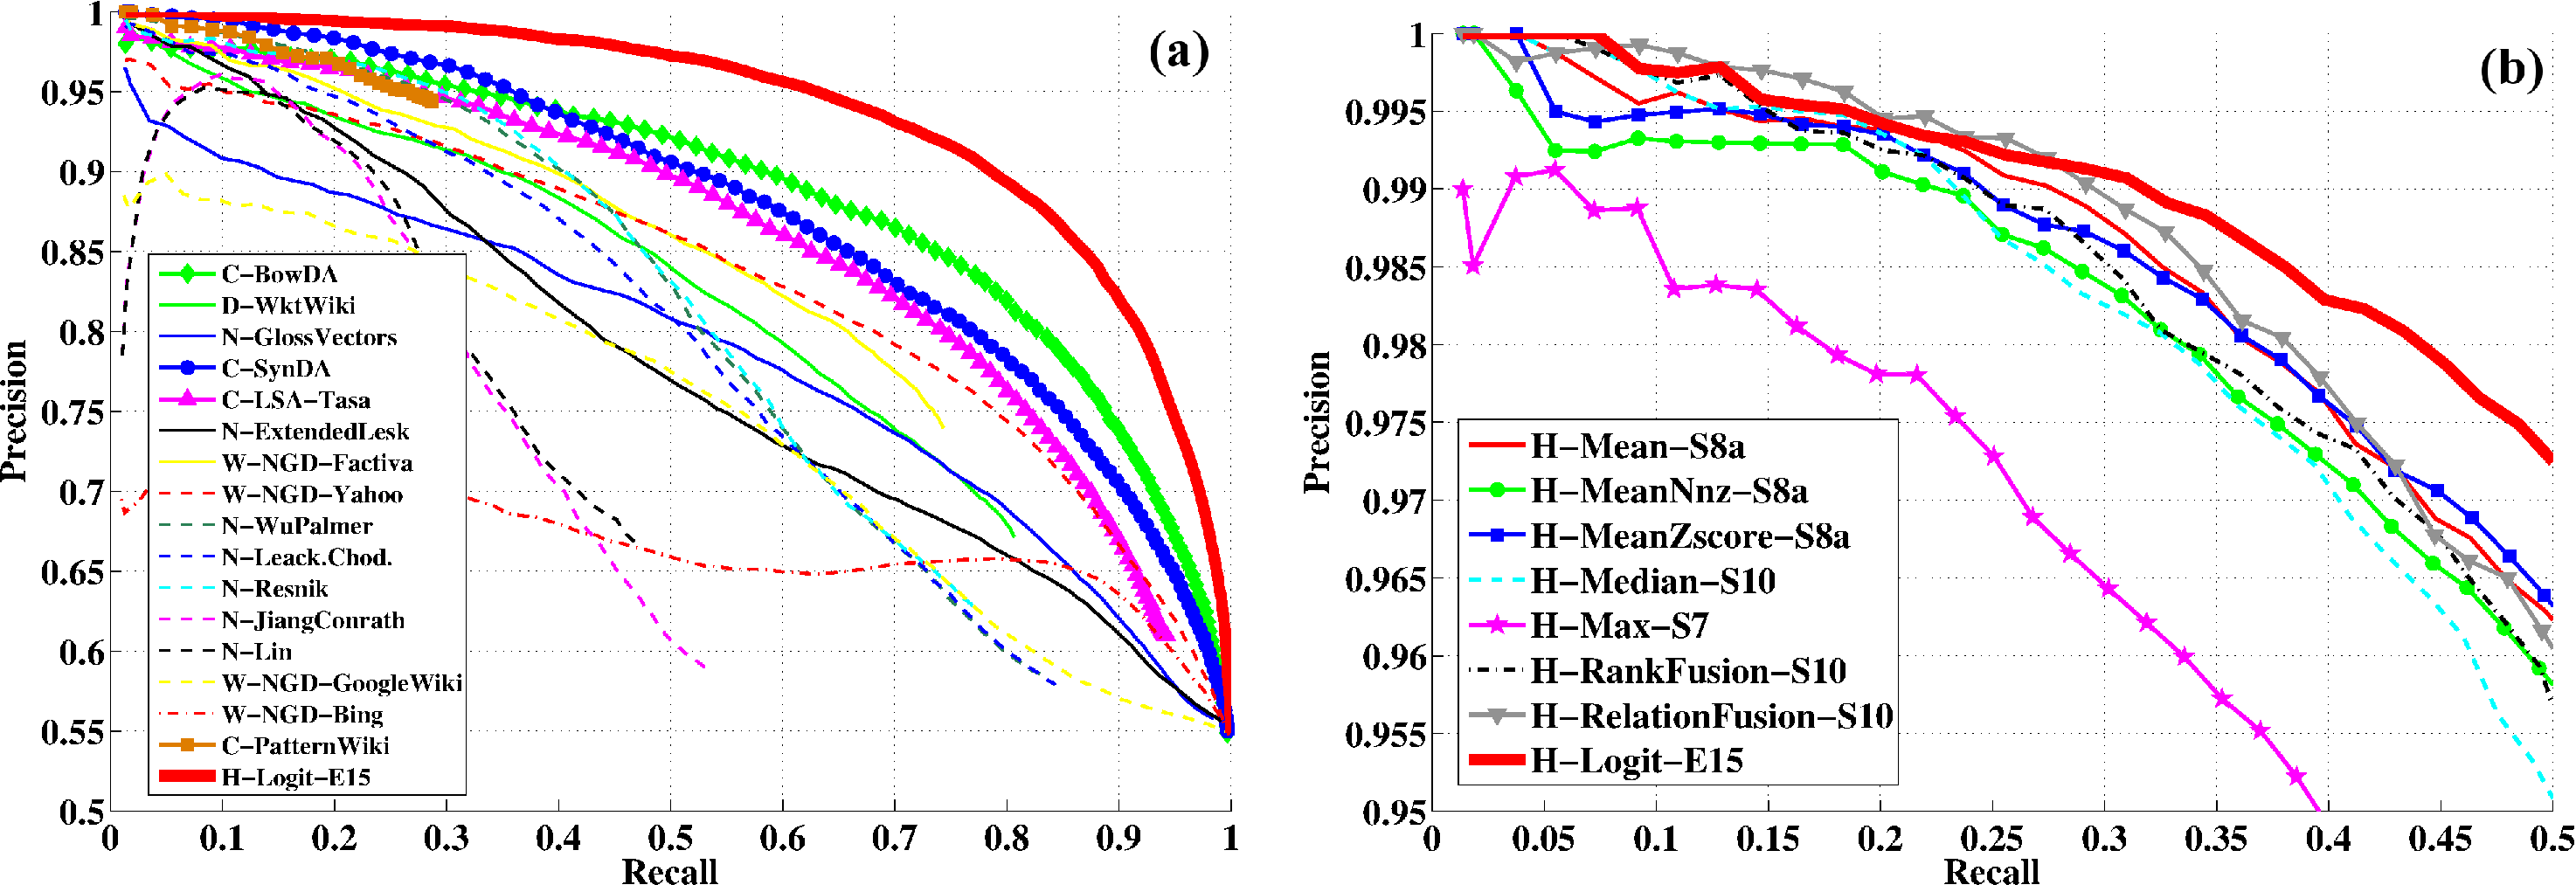
\includegraphics[width=1.0\textwidth]{figures/pr}
		\caption{Precision-Recall graphs calculated on the BLESS dataset of (a) 16 single measures and the best hybrid
measure H-Logit-E15; (b) 8 hybrid measures.}
\end{figure}
	
\end{frame}

\begin{frame}
 \frametitle{Hybrid Similarity Measure Logit-E15}
	\begin{figure}
	\centering
		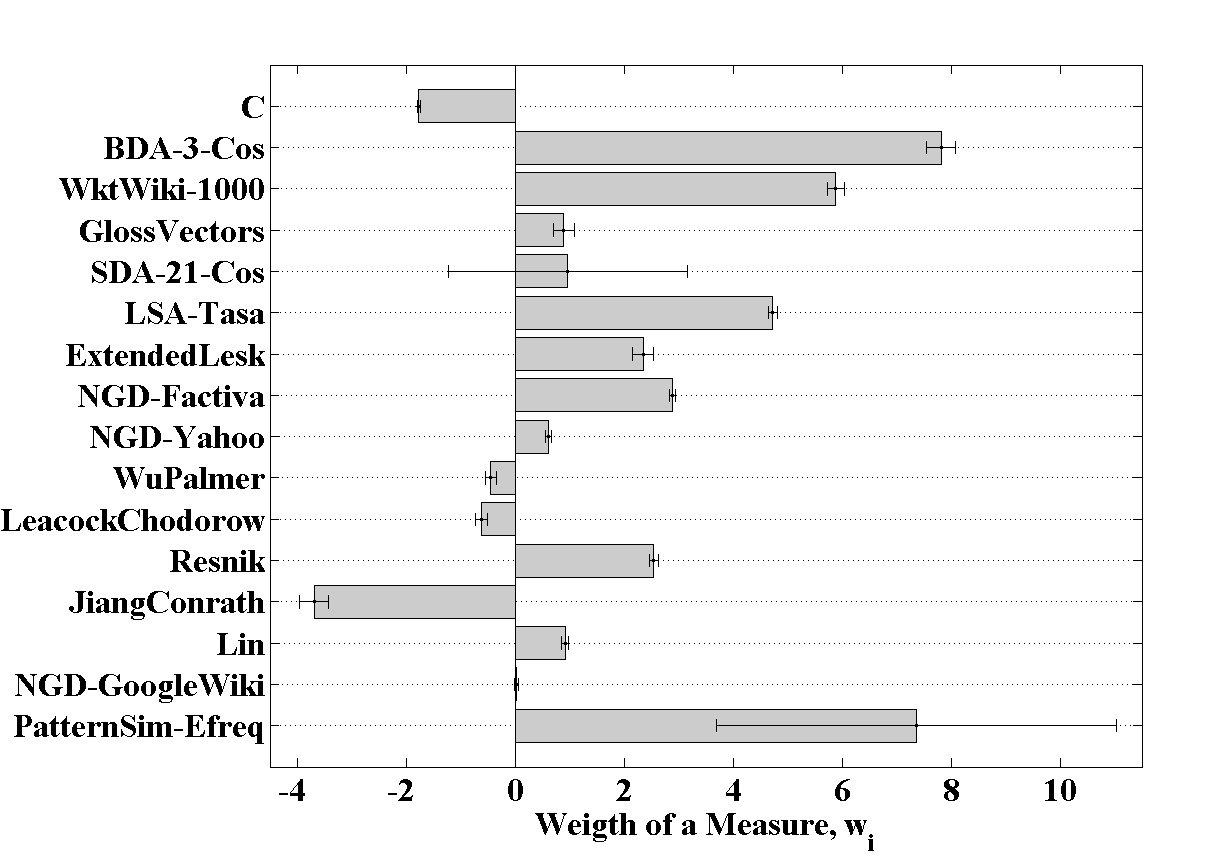
\includegraphics[width=0.7\textwidth]{figures/logit-e15-bless-errorbars}
		\caption{Weights of the features used by the hybrid measure Logit-E15 as learned from the BLESS training dataset. }
\end{figure}
	
\end{frame}

\begin{frame}
\frametitle{Hybrid Similarity Measure Logit-E15}
\begin{figure}
\centering
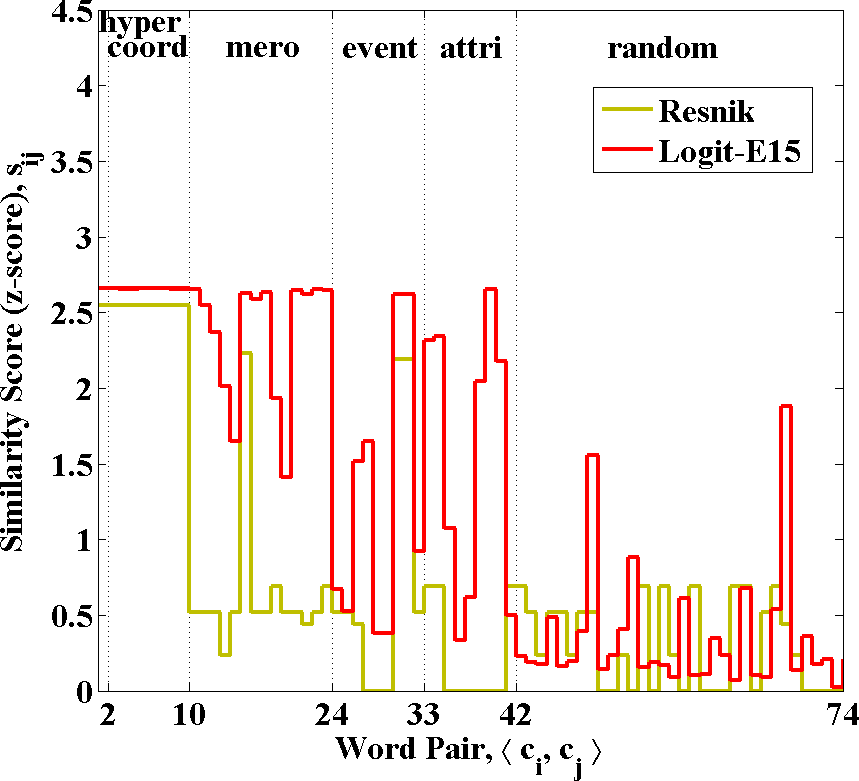
\includegraphics[width=0.32\textwidth]{figures/acacia-resnik} 
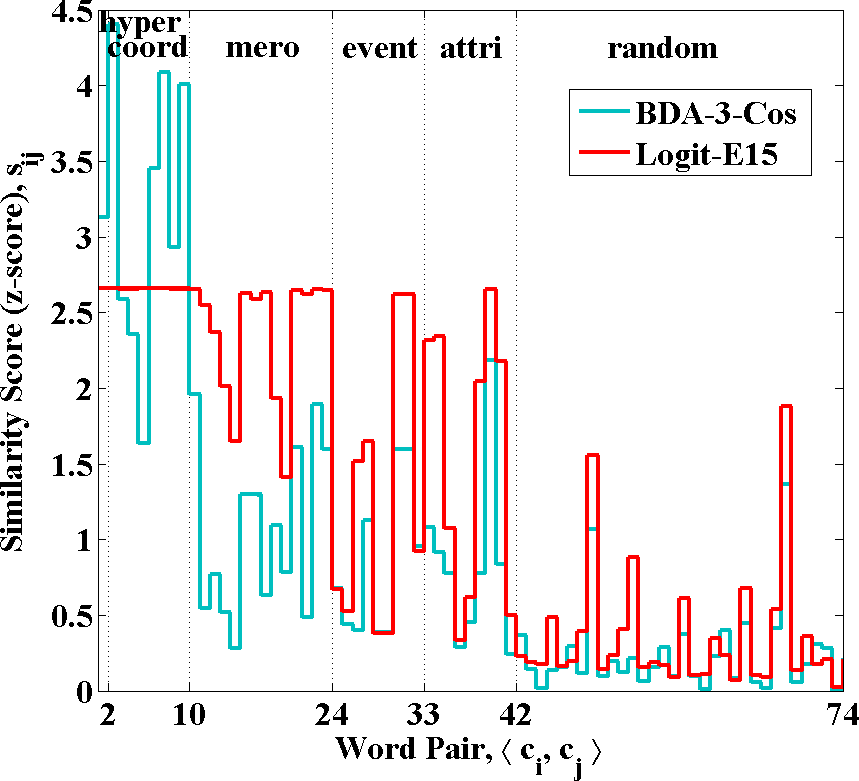
\includegraphics[width=0.32\textwidth]{figures/acacia-bda}
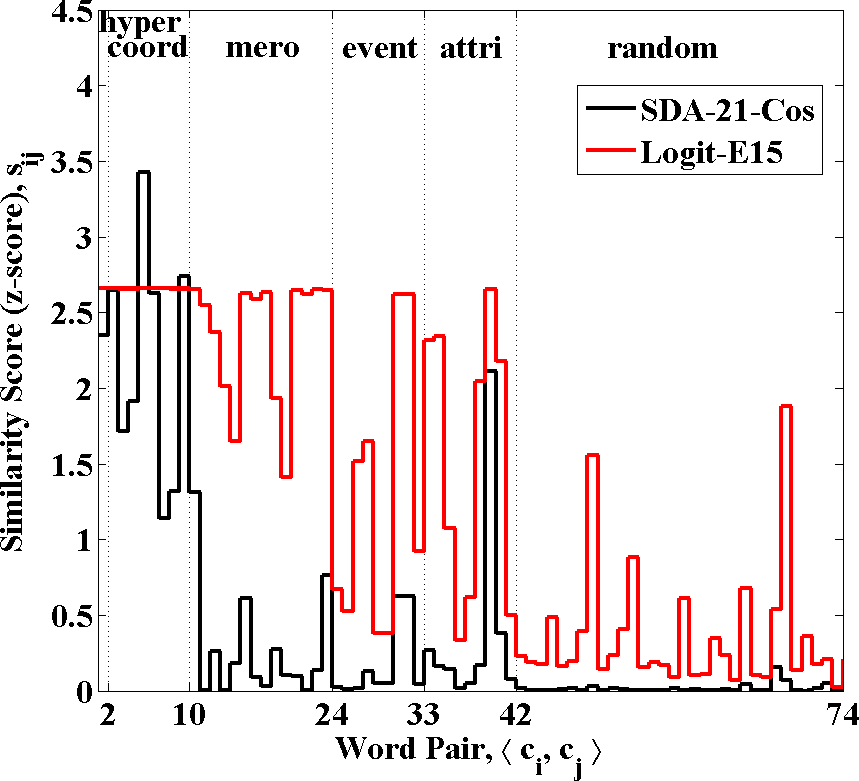
\includegraphics[width=0.32\textwidth]{figures/acacia-sda}

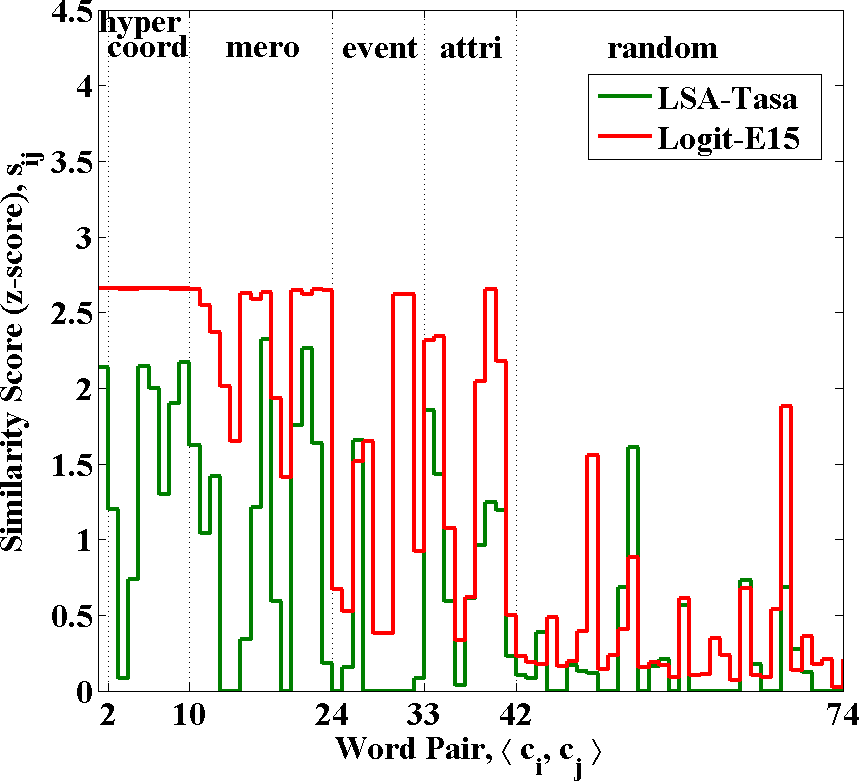
\includegraphics[width=0.32\textwidth]{figures/acacia-lsa}
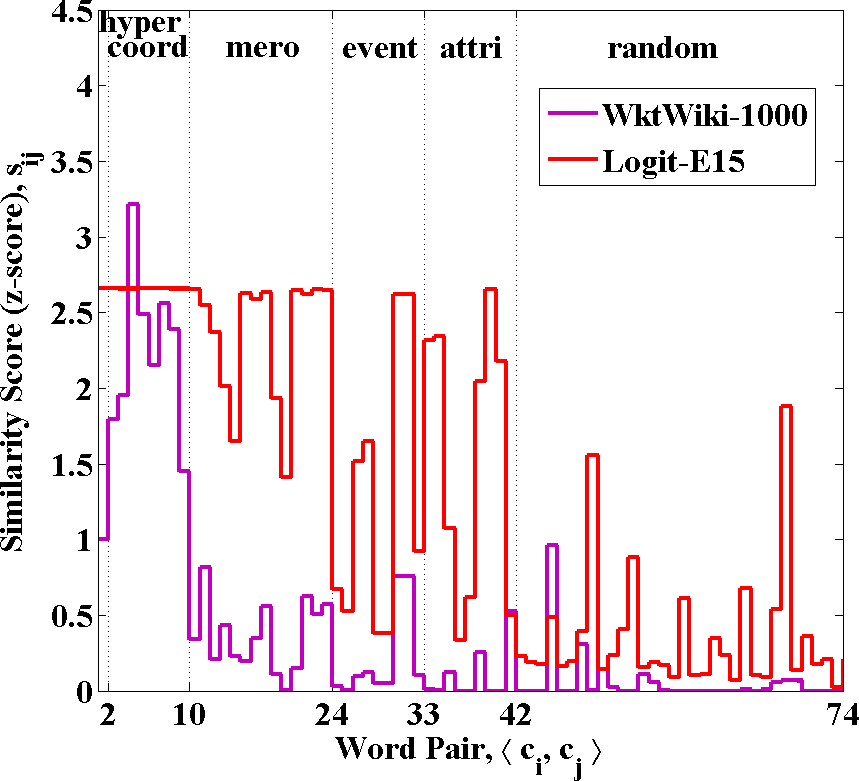
\includegraphics[width=0.32\textwidth]{figures/acacia-ww}
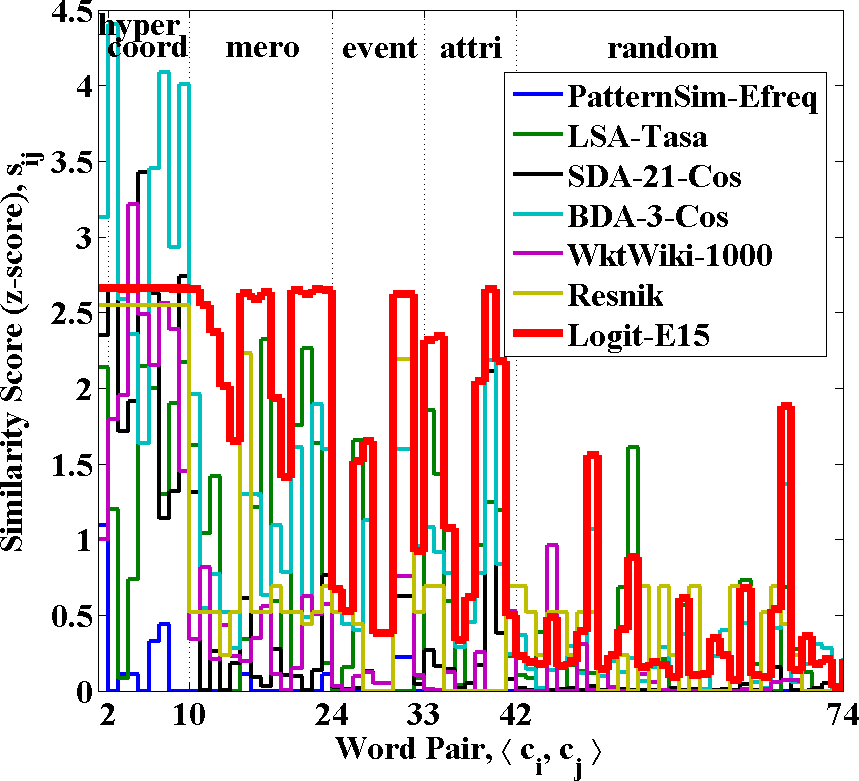
\includegraphics[width=0.32\textwidth]{figures/acacia}
\caption{ Similarity scores between 74 words related to word ``acacia'' calculated by single measures and hybrid measure Logit-E15 (z-scores). }
\label{fig:hybrid-complimentary-discussion}
\end{figure}

\end{frame}

%%%%%%%%%%%%%%%%%%%%%%%%%%%%%%%%%%%%%%%%%%%%%%%%%
\subsection{Conclusion}
%\subsection{}

%%%%%%%%%%%%%%%%%%%%%%%%%%%%%%%%%%%%%%%%%%%%%%%%%
\begin{frame}
\frametitle{Conclusion:}

\begin{itemize}
  
%\item We designed and studied several
%hybrid similarity measures in the context of semantic relation extraction.

%\item We have undertaken \textbf{a study} of 16 baseline measures, 8
%combination methods, and 3 measure selection techniques.

\item The \textbf{proposed hybrid measures}:


\begin{itemize}
  \item use all 5 main types of baseline measures;
  \item outperform the single measures on all datasets.
\end{itemize}  

  
\item The \textbf{best results} were provided by
\begin{itemize}
  \item  a combination of 15  corpus-, web-, network-, and definition-based measures
\item with Logistic Regression 
%\item $\rho= 0.870$, $P(20)=0.987$, $R(50)=0.814$.
\end{itemize}
 
\end{itemize}


\end{frame}

\section{Applications}
\subsection{}
\begin{frame}
\frametitle{Applications of Semantic Similarity Measures}

\begin{itemize}
  \item \textbf{Lexico-Semantic Search Engine}
  \begin{itemize}
    \item \url{http://serelex.cental.be/}
    \item (Panchenko, Morozova and Naets, 2012)
    \end{itemize}
    
  \item \textbf{Short Text Classification} (Panchenko et al., submitted to ECIR 2013)
  
  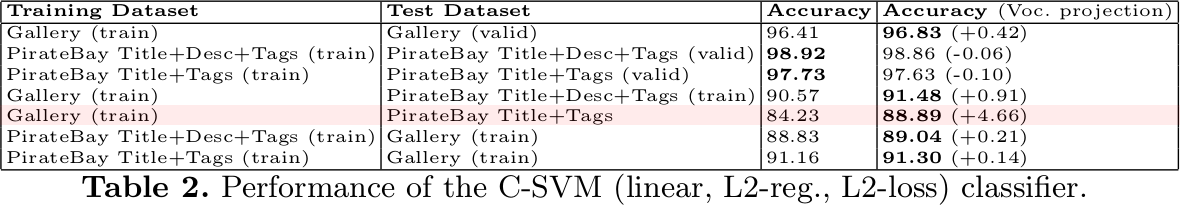
\includegraphics[width=0.88\textwidth]{figures/stc}
  
  \item \textbf{Query Expansion} 
  
  \item \textbf{Term/Text Clustering} 
\end{itemize}
\end{frame}

\begin{frame}
\frametitle{}

\Huge \bf Thank you! Questions?
\end{frame}
\end{document}